\section{Condições de Contorno}

Em

\begin{equation}
 \label{cap6:sec5:eq2}
 x = 0 \Rightarrow u\,(0) = 0
 \left\{
 \begin{array}{l}
  \mbox{c c essencial} \\
  \mbox{c c cinemática} \\
  \mbox{c c Dirichlet}
 \end{array}
 \right.
\end{equation}

Em

\begin{equation}
 \label{cap6:sec5:eq3}
 x = L \Rightarrow F\,(L) = c \, L \, \frac{du}{dx} \, (L) = 0
 \left\{
 \begin{array}{l}
  \mbox{c c natural} \\
  \mbox{c c dinâmica} \\
  \mbox{c c de Neuman}
 \end{array}
 \right.
\end{equation}

Problemas de Sturm-Liouville

\begin{equation}
 \label{cap6:sec5:eq4}
 \mbox{ \framebox{ $ - \displaystyle \frac{d}{dx} \, \left(c \, \displaystyle \frac{du}{dx} \right) + q \, u = f $ } }
\end{equation}

\begin{example}

Suponha a equação:

\begin{equation}
 \left\{
 \begin{array}{l}
  - 2 \, y''(x) + y \, (x) = e^{-0.2 \, x} \\
  \mbox{B.c.} \\
  \begin{array}{lll}
   \qquad y\,(0) & = & 1 \\
   \qquad y'(10) & = & -y \, (10)
  \end{array}
 \end{array}
 \right.
\end{equation}

Resolva por diferenças finitas

\begin{figure}[htb]
 \centering
 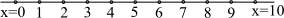
\includegraphics[scale=1.0]{capitulos/capitulo6/figuras/cond_contorno1.png}
 \caption{?}
 \label{fig:cond_contorno1}
\end{figure}

Em

\[
 x = x_i \Rightarrow - 2 \, \left[ \frac{y_{i-1} - 2 \, y_i + y_{i+1}}{h^2} \right] + y_i = e^{-0.2 \, x_i}
\]

\[
 \begin{array}{lll}
  h = 1 & \Rightarrow & -2 \, y_{i-1} + 4 \, y_i - 2 \, y_{i+1} + y_i = e^{-0.2 \, x_i} \\
        & \Rightarrow & \underbrace{\mbox{\framebox{$-2$}}}_{i-1}-\underbrace{\mbox{\framebox{$+5$}}}_{i}-\underbrace{\mbox{\framebox{$-2$}}}_{i+1}
 \end{array}
\]

Aplique nos pontos \esp{1, \, 2, \, \ldots , \, 9}

\[
 \begin{array}{clllllll}
  \mbox{Em } x = 1 & \Rightarrow & -2\,y_0 & +5\,y_1 & -2\,y_2 & & & = e^{-0.2} \nonumber \\
  \mbox{Em } x = 2 & \Rightarrow &         & -2\,y_1 & +5\,y_2 & -2\,y_3 & & = e^{-0.4} \nonumber \\
  \vdots & & & & \vdots & \nonumber \\
  \mbox{Em } x = 9 & \Rightarrow &         &         & -2\,y_8 & +5\,y_9 & -2\,y_{10} & = e^{-1.8} \nonumber \\
 \end{array}
\]

\end{example}
